\chapter{Estado del arte y tecnologías}
\label{chap:estado-arte}

Este capítulo presenta los fundamentos conceptuales y tecnológicos de la
propuesta. En primer lugar, se revisan la programación basada en bloques,
Blockly y los principios de los lenguajes de dominio específico y de la
ingeniería dirigida por modelos. A continuación, se describen EMF, Ecore y
Xtext, tecnologías utilizadas en el desarrollo de Model2Blockly. Después se
analizan los trabajos relacionados sobre DSLs basados en bloques y se compara
la propuesta con ellos para precisar su posicionamiento. Finalmente, se explica
la relación entre las tecnologías seleccionadas dentro de la cadena de
generación planteada.

\section{Programación basada en bloques}
\label{sec:block-based}

La programación basada en bloques sustituye parte de la escritura textual por
piezas visuales. Estas piezas representan instrucciones, expresiones o
estructuras de control. El entorno define cómo se pueden conectar, por lo que se
evitan muchas combinaciones sintácticamente incorrectas. Además, el usuario puede
ver qué construcciones están disponibles. Por esta razón, los entornos de bloques
se usan con frecuencia para introducir la programación a usuarios noveles
\cite{resnick2009scratch,lin2021landscape}. Herramientas de análisis como
Dr. Scratch muestran además que los programas de bloques pueden inspeccionarse
y evaluarse automáticamente, lo que refuerza su interés como representación
estructurada y no solo como interfaz gráfica \cite{moreno2015drscratch}.

Los bloques no son solo una forma gráfica de mostrar código. La forma en que el
usuario representa y manipula las construcciones del lenguaje influye en su forma
de programar \cite{weintrop2018modalities}. Por eso, al diseñar un lenguaje de
bloques hay que decidir qué conceptos serán bloques, qué parámetros serán campos,
cómo se organizará la paleta, qué conexiones serán válidas y qué restricciones se
mostrarán al usuario.

La Figura \ref{fig:blockly-music-maker} muestra un ejemplo de esta forma de
programación en Music Maker, una aplicación web desarrollada en el codelab
oficial de Blockly \cite{blocklyGettingStartedCodelab}. En el modo de edición,
el usuario construye un programa encajando un bloque que reproduce la nota D4
dentro de una estructura que repite la acción tres veces. La forma de las piezas
expresa la relación estructural entre las instrucciones, mientras que los campos
permiten configurar la repetición y la nota sin escribir código textual. El modo
de reproducción presenta los botones de la aplicación sobre los que se ejecutan
los programas musicales definidos mediante bloques.

\begin{figure}[htbp]
  \centering
  \begin{minipage}[t]{0.47\textwidth}
    \centering
    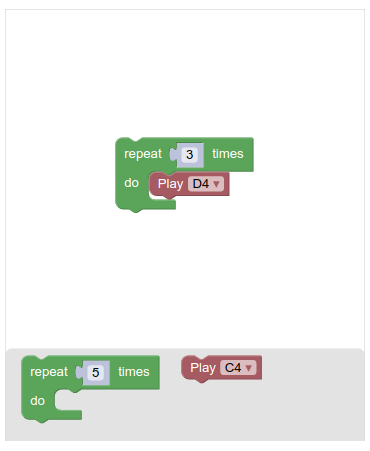
\includegraphics[width=\textwidth]{assets/blockly/d4_three_times.png}

    \small (a) Edición del programa mediante bloques
  \end{minipage}
  \hfill
  \begin{minipage}[t]{0.47\textwidth}
    \centering
    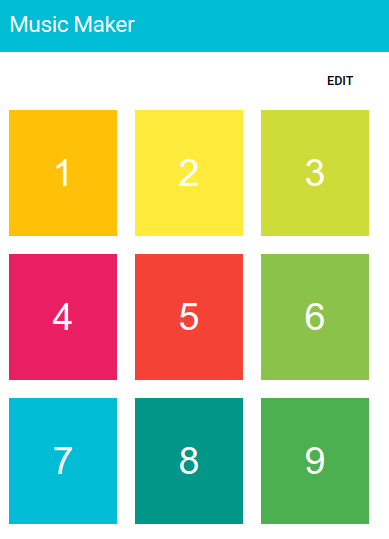
\includegraphics[width=\textwidth]{assets/blockly/play_mode.png}

    \small (b) Interfaz de reproducción de Music Maker
  \end{minipage}
  \caption{Edición y reproducción de un programa basado en bloques en Music
  Maker. Fuente: codelab oficial de Blockly \cite{blocklyGettingStartedCodelab}}
  \label{fig:blockly-music-maker}
\end{figure}

En este TFM, la programación por bloques se entiende como una sintaxis concreta
visual, es decir, como la forma visible con la que el usuario manipula un
lenguaje de dominio específico. El usuario final no necesita conocer la
implementación JavaScript del editor ni la estructura interna del metamodelo;
interactúa con un conjunto de bloques que representan conceptos del dominio.
Esta idea conecta directamente con la motivación del trabajo: crear lenguajes
de bloques para diferentes dominios sin programar manualmente cada editor desde
cero.

\section{Blockly}
\label{sec:blockly}

Blockly es una biblioteca web de código abierto para construir editores basados
en bloques. La documentación oficial describe Blockly como una biblioteca que
permite integrar un editor de código visual en una aplicación web; el
desarrollador define los bloques y la semántica asociada, mientras que la
biblioteca proporciona la infraestructura de interacción visual, arrastre,
encaje, paleta y serialización \cite{blocklyWhatIs,blocklyDocs}.

La biblioteca permite definir bloques con campos, entradas de valor, entradas
de sentencias, conexiones previas y posteriores, colores, tooltips y
generadores de código. También permite organizar los bloques en categorías de
paleta o \emph{toolbox}, y serializar el estado del área de trabajo o
\emph{workspace} \cite{blocklyGoogleDevelopers}. Estas capacidades hacen que
Blockly sea una base adecuada para construir lenguajes visuales específicos,
pero no eliminan la necesidad de definir manualmente la configuración de cada
dominio.

Antes de definir elementos específicos del dominio, el desarrollador debe
cargar las dependencias, proporcionar un contenedor HTML e inicializar el
espacio de trabajo. El Listado \ref{lst:blockly-infraestructura-minima} resume esta
infraestructura mínima siguiendo el codelab oficial
\cite{blocklyGettingStartedCodelab}.

\begin{lstlisting}[style=tfmhtml, caption={Infraestructura mínima para crear un espacio de trabajo Blockly}, label={lst:blockly-infraestructura-minima}]
<script src="https://unpkg.com/blockly/blockly_compressed.js"></script>
<script src="https://unpkg.com/blockly/blocks_compressed.js"></script>
<script src="https://unpkg.com/blockly/javascript_compressed.js"></script>
<script src="https://unpkg.com/blockly/msg/en.js"></script>

<div id="blocklyDiv"></div>

Blockly.inject("blocklyDiv", {"toolbox": toolbox});
\end{lstlisting}

El Listado \ref{lst:blockly-music-maker-config} muestra un ejemplo reducido de
esa configuración, tomado del codelab oficial Music Maker
\cite{blocklyGettingStartedCodelab}. El primer objeto define un bloque con un
campo desplegable para seleccionar una nota y con conexiones anterior y
posterior. El segundo determina qué tipos de bloque aparecen en la paleta.
Aunque se habla habitualmente de definiciones JSON, en este caso se expresan
como objetos JavaScript cuyos valores son serializables como JSON.

\begin{lstlisting}[style=tfmjavascript, caption={Definición de un bloque y configuración mínima de una paleta en Blockly}, label={lst:blockly-music-maker-config}]
Blockly.common.defineBlocksWithJsonArray([{
  "type": "play_sound",
  "message0": "Play %1",
  "args0": [{
    "type": "field_dropdown",
    "name": "VALUE",
    "options": [
      ["C4", "sounds/c4.m4a"],
      ["D4", "sounds/d4.m4a"]
    ]
  }],
  "previousStatement": null,
  "nextStatement": null,
  "colour": 355
}]);

const toolbox = {
  "kind": "flyoutToolbox",
  "contents": [
    {"kind": "block", "type": "controls_repeat_ext"},
    {"kind": "block", "type": "play_sound"}
  ]
};
\end{lstlisting}

La Figura \ref{fig:blockly-music-maker-toolbox} muestra el editor resultante: la
paleta ofrece el bloque de repetición y el bloque musical, que pueden
arrastrarse al espacio de trabajo para construir el programa.

\begin{figure}[htbp]
  \centering
  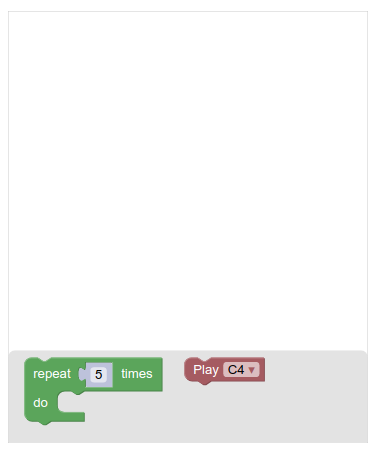
\includegraphics[width=0.48\textwidth]{assets/blockly/workspace_with_toolbox.png}
  \caption{Espacio de trabajo y paleta obtenidos tras registrar el bloque
  \texttt{play\_sound}. Fuente: codelab oficial de Blockly
  \cite{blocklyGettingStartedCodelab}}
  \label{fig:blockly-music-maker-toolbox}
\end{figure}

Aunque el editor resultante solo ofrece un bucle y una operación musical, su
construcción exige gestionar dependencias, preparar el contenedor, configurar
el espacio de trabajo y declarar manualmente la estructura, los campos, las conexiones y
la paleta. Todavía habría que añadir el generador de código y la lógica de
ejecución. Este esfuerzo crece con el número de conceptos y restricciones del
dominio y se repite para cada editor. La Figura
\ref{fig:blockly-music-maker}, presentada en la sección anterior, muestra cómo
el usuario combina posteriormente esos bloques para definir el comportamiento
de Music Maker.

El problema que aborda este TFM aparece precisamente en ese punto. Si se desea
crear un editor Blockly para un dominio de planificación, otro para un dominio
de storytelling y otro para un dominio de robótica, gran parte del trabajo se
repite: declarar bloques, campos, categorías, conexiones, validaciones y
generadores. El enfoque propuesto consiste en generar esos elementos a partir
de una descripción abstracta del dominio. Así, Blockly se utiliza como
plataforma de ejecución visual, pero la especificación del lenguaje se mantiene
en un nivel de metamodelo o DSL.

\section{Lenguajes de dominio específico e ingeniería dirigida por modelos}
\label{sec:dsml-mde}

Un lenguaje de dominio específico ofrece conceptos y notaciones adaptados a una
familia concreta de problemas. A diferencia de un lenguaje de propósito general,
un DSL permite usar términos propios del dominio. En enfoques basados en
metamodelado, un DSL suele tener una sintaxis abstracta, definida mediante un
metamodelo, y una o varias sintaxis concretas con las que trabaja el usuario
\cite{sal2024dsl,wasowski2023dsl}.

La ingeniería dirigida por modelos ofrece un marco para esta separación. En MDE,
los modelos son artefactos principales del desarrollo. Se usan para especificar,
diseñar, analizar, transformar y generar software \cite{brambilla2017modelDriven}.
En la industria, algunas motivaciones para usar MDE son reducir tiempo de
desarrollo, reutilizar soluciones y mejorar la calidad
\cite{brambilla2017modelDriven,hutchinson2014industry,akdur2018survey}.
Estas ideas encajan con este TFM: usar un generador para producir editores
Blockly en vez de programar cada editor desde cero.

En el ámbito del modelado, existen también estándares generales como UML y OCL.
UML define una notación gráfica estandarizada para visualizar, especificar,
construir y documentar sistemas software, mientras que OCL proporciona un
lenguaje formal para expresar restricciones sobre modelos \cite{omgUml,omgOcl}.
Estos estándares son relevantes como contexto, pero el presente TFM no propone
un perfil UML ni una integración completa de OCL. La decisión tomada es más
concreta: usar un metamodelo como descripción abstracta del dominio,
enriquecerlo con información sobre la sintaxis visual y derivar a partir de ella
una sintaxis concreta basada en bloques. En este trabajo, esta función se
implementa mediante Ecore, tecnología que se presenta en la Sección
\ref{sec:emf-ecore}.
El DSL textual del proyecto se entiende como una segunda ruta de autoría para
diseñadores de lenguajes: permite describir la estructura del editor Blockly de
forma más compacta y normalizarla al mismo modelo intermedio.

La experiencia acumulada en lenguajes específicos de dominio muestra además que
las herramientas de modelado pueden elevar el nivel de abstracción al expresar
soluciones directamente con conceptos del dominio y generar artefactos a partir
de esos modelos \cite{luoma2004dsm}. Esta idea coincide con la motivación de
Model2Blockly: que el usuario defina los conceptos del dominio y que la
infraestructura genere el editor visual correspondiente.

En este proyecto, la sintaxis basada en bloques se considera una sintaxis
concreta visual del dominio. El metamodelo Ecore describe qué conceptos existen
y cómo se relacionan; las anotaciones aportan información de presentación que
Ecore no expresa de forma nativa; la ruta textual \texttt{.m2b} puede escribir
la definición del lenguaje de bloques en un formato más breve. El generador
produce la configuración Blockly que implementa la sintaxis visual usada por el
usuario final.

\section{EMF y Ecore}
\label{sec:emf-ecore}

Eclipse Modeling Framework (EMF) es una infraestructura de modelado para definir
modelos estructurados y generar código a partir de ellos. Ecore es el
metamodelo central de EMF y permite representar paquetes, clases, atributos,
referencias, tipos de datos, herencia y cardinalidades
\cite{emfOverview,steinberg2008emf}. En la práctica, Ecore proporciona una
forma compacta y ampliamente utilizada de describir la estructura abstracta de
un dominio.

En este TFM, Ecore cumple tres funciones. Primero, describe la estructura del
dominio: las clases son conceptos, los atributos son propiedades y las
referencias son relaciones. Segundo, permite obtener información para la sintaxis
de bloques: una clase puede ser un tipo de bloque, un atributo puede ser un campo
y una referencia de contención puede ser una entrada para bloques hijos. Tercero,
Ecore permite añadir anotaciones de presentación, como etiquetas, colores,
categorías o tooltips.

La Figura \ref{fig:ecore-metamodelo-simplificado} representa el fragmento del
metamodelo Ecore relevante para estas funciones. Se omiten algunos tipos
intermedios, como \texttt{ENamedElement} y \texttt{ETypedElement}, para mantener
legible el diagrama.

\begin{figure}[H]
  \centering
  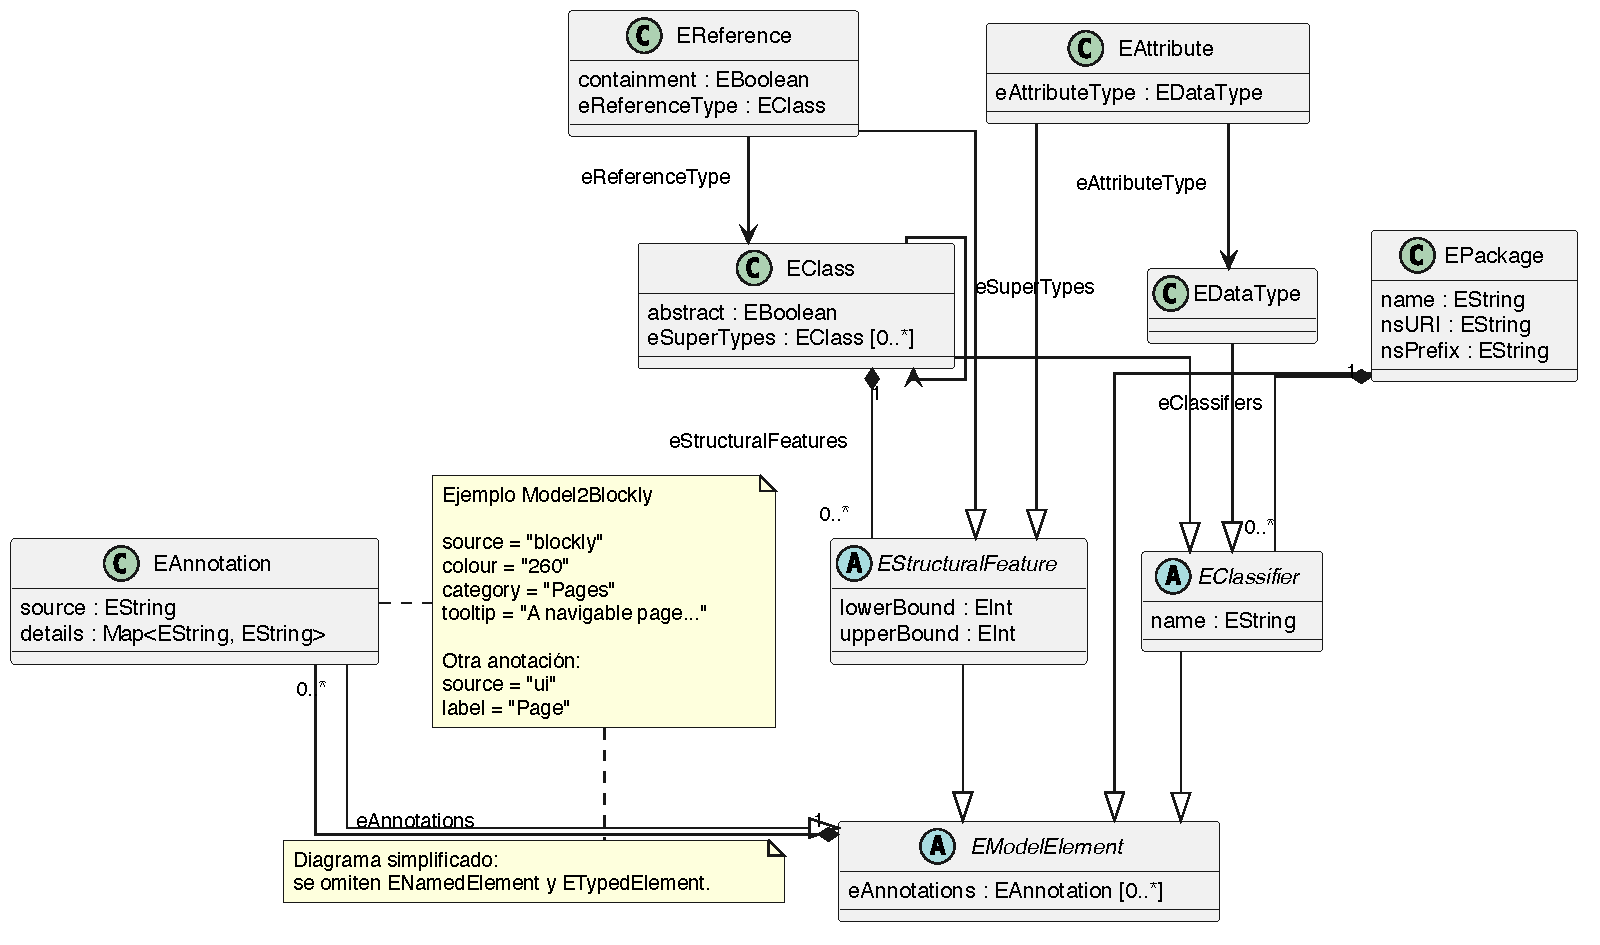
\includegraphics[width=\textwidth]{assets/uml/uml.pdf}
  \caption{Fragmento simplificado del metamodelo Ecore y uso de anotaciones en
  Model2Blockly}
  \label{fig:ecore-metamodelo-simplificado}
\end{figure}

Un \texttt{EPackage} agrupa los clasificadores del dominio. Entre ellos, una
\texttt{EClass} representa un concepto y puede contener características
estructurales: los \texttt{EAttribute} almacenan valores tipados y las
\texttt{EReference} relacionan instancias de clases, con la posibilidad de
marcar una relación como contención. Los límites inferior y superior expresan
la cardinalidad de cada característica. Estos elementos heredan, directa o
indirectamente, de \texttt{EModelElement}, que permite asociar instancias de
\texttt{EAnnotation}. Cada anotación identifica su propósito mediante
\texttt{source} y almacena pares clave--valor en \texttt{details}; Model2Blockly
utiliza este mecanismo para incorporar información de sintaxis visual sin
alterar la estructura abstracta del dominio. En el ejemplo de la figura, la
anotación con \texttt{source="blockly"} define \texttt{colour},
\texttt{category} y \texttt{tooltip}, mientras que una anotación separada con
\texttt{source="ui"} proporciona la etiqueta visible mediante \texttt{label}.

Esta capacidad de separar estructura e información de presentación es esencial
para el trabajo. No todos los detalles de un editor Blockly existen de forma
natural en un metamodelo Ecore: por ejemplo, el color de un bloque o la
organización de la paleta son decisiones de sintaxis concreta. Por ello, el
proyecto permite enriquecer el metamodelo con anotaciones específicas, sin
perder la posibilidad de generar un editor básico a partir de la estructura
Ecore.

\section{Xtext}
\label{sec:xtext}

Xtext es un framework de Eclipse para el desarrollo de lenguajes textuales
específicos de dominio. A partir de una gramática, Xtext genera infraestructura
de análisis sintáctico, un modelo abstracto basado en EMF y soporte de edición
como resaltado de sintaxis, navegación, autocompletado y marcadores de error
\cite{xtextProject,bettini2013xtext,bettini2015xsemantics}. Estas
características lo hacen adecuado para construir una ruta textual alternativa a
la edición directa de metamodelos Ecore.

Conviene distinguir dos momentos en el funcionamiento de Xtext. En primer
lugar, durante la construcción de la herramienta, el desarrollador escribe una
gramática que describe las palabras clave, las reglas y las referencias del
lenguaje. Xtext procesa esa gramática y genera el analizador, la infraestructura
EMF y los servicios del editor. En segundo lugar, durante el uso de la
herramienta, ese analizador lee cada fichero escrito en el nuevo lenguaje y
construye una instancia de su modelo abstracto. Por lo tanto, Xtext no genera el
editor Blockly directamente: genera la infraestructura que permite comprender
una especificación textual, que después Model2Blockly transforma.

La Figura \ref{fig:funcionamiento-general-xtext} resume este mecanismo. La
gramática determina qué textos son válidos y cómo se relacionan con los
conceptos del modelo. A partir de ella se obtienen el parser y los servicios de
edición. Cuando el autor escribe una especificación, el parser construye un
grafo de objetos EMF; el enlazado resuelve nombres que hacen referencia a otros
elementos y el validador comunica los problemas detectados. Una transformación
posterior puede entonces consumir ese modelo sin volver a interpretar el texto.

\begin{figure}[htbp]
  \centering
  \resizebox{\textwidth}{!}{%
  \begin{tikzpicture}[
      node distance=0.75cm and 0.38cm,
      box/.style={draw=black!55, rounded corners=2pt, minimum width=2.18cm,
        minimum height=0.92cm, align=center, font=\small, inner sep=5pt},
      sourcebox/.style={box, fill=green!8},
      xtextbox/.style={box, fill=blue!7},
      commonbox/.style={box, fill=orange!10},
      arrow/.style={-{Latex[length=2.4mm]}, thick, draw=black!70},
      control/.style={-{Latex[length=2.2mm]}, dashed, thick, draw=black!55}
    ]
    \node[sourcebox] (dsl) {Especificación\\textual \texttt{.m2b}};
    \node[xtextbox, right=of dsl] (parser) {Parser, enlazado\\y validación};
    \node[xtextbox, right=of parser] (model) {Modelo abstracto\\basado en EMF};
    \node[commonbox, right=of model] (transformation)
      {Transformación de\\Model2Blockly};
    \node[commonbox, right=of transformation] (editor)
      {Editor Blockly\\generado};
    \node[sourcebox, above=0.55cm of parser] (grammar) {Gramática Xtext};

    \draw[control] (grammar.south) -- (parser.north);
    \draw[arrow] (dsl) -- (parser);
    \draw[arrow] (parser) -- (model);
    \draw[arrow] (model) -- (transformation);
    \draw[arrow] (transformation) -- (editor);
  \end{tikzpicture}%
  }
  \caption{Funcionamiento general de Xtext y su aplicación en Model2Blockly}
  \label{fig:funcionamiento-general-xtext}
\end{figure}

En este proyecto, Xtext se usa para definir el lenguaje textual
\texttt{.m2b}. El Listado \ref{lst:xtext-m2b-breve} ilustra su nivel de
abstracción: el autor declara conceptos del dominio, propiedades y relaciones,
en lugar de programar directamente llamadas a la API JavaScript de Blockly.

\begin{lstlisting}[style=tfmm2b, caption={Ejemplo breve de una definición textual \texttt{.m2b}}, label={lst:xtext-m2b-breve}]
// Define el nombre del dominio que se transformara.
domain BasicStructure
// Declara una clase concreta y desactiva los campos en linea.
class Board inputsInline false {
  // Define un atributo de texto opcional con valor inicial.
  attribute name : string [0..1] default "Sprint board"
  // Expresa una contencion de uno a cuatro elementos.
  contains WorkItem items [1..4]
} // Finaliza la declaracion de Board.
// Declara el tipo abstracto usado por la contencion.
abstract class WorkItem inputsInline false {
} // Finaliza la declaracion de WorkItem.
\end{lstlisting}

La declaración \texttt{class Board} representa un concepto que podrá convertirse
en un tipo de bloque; \texttt{name} aporta una propiedad editable e
\texttt{items} expresa una relación jerárquica con cardinalidad. Xtext
comprueba que la entrada respeta la gramática y que nombres como
\texttt{Board} y \texttt{WorkItem} se pueden resolver. El resultado es un
modelo EMF que la cadena de Model2Blockly puede transformar posteriormente.
Este mecanismo concreto se desarrolla desde el punto de vista arquitectónico
en la Sección \ref{sec:ruta-xtext} y desde el punto de vista de implementación
en la Sección \ref{sec:implementacion-xtext}.

La ruta Xtext no sustituye, por lo tanto, a la ruta Ecore; la complementa. Ecore
resulta adecuado cuando ya existe un metamodelo EMF o cuando se quiere mantener
la definición del dominio dentro de dicho ecosistema. La ruta \texttt{.m2b}
resulta útil cuando se desea reunir en un fichero legible la estructura del
dominio y las decisiones de sintaxis concreta, como etiquetas, colores,
widgets, organización de la paleta y plantillas de código. La convergencia en
\texttt{EditorSpec} evita mantener dos generadores diferentes.

\section{Xtend}
\label{sec:xtend}

Xtend es un lenguaje de programación estáticamente tipado del ecosistema Xtext.
Su sintaxis parte de Java, pero añade construcciones más concisas, como
inferencia de tipos, métodos de extensión, expresiones lambda, expresiones
\texttt{switch} y plantillas de texto. El compilador de Xtend traduce los
ficheros \texttt{.xtend} a código fuente Java, por lo que el código resultante se
ejecuta sobre la JVM y puede utilizar directamente clases y bibliotecas Java
\cite{xtendDocs}.

Para la generación de código resultan especialmente útiles las expresiones de
plantilla. Una plantilla se delimita mediante triples comillas simples y permite
insertar expresiones entre los caracteres \texttt{«} y \texttt{»}. Xtend evalúa
esas expresiones, incorpora su representación textual y aplica reglas de
indentación que ayudan a mantener legibles tanto la plantilla como la salida
generada \cite{xtendDocs}. El Listado \ref{lst:xtend-plantilla} muestra un
fragmento simplificado, basado en el generador del proyecto.

\begin{lstlisting}[style=tfmxtend, caption={Ejemplo de una plantilla Xtend usada para generar JavaScript}, label={lst:xtend-plantilla}]
def String generateBlocksJs(EditorSpec spec) '''
  // Block definitions for domain "«spec.domainName»".
  window.BLOCKLY_BLOCKS = «generateBlocksArray(spec)»;
'''
\end{lstlisting}

En el ejemplo, \texttt{def} declara un método y la plantilla constituye su
resultado. Las expresiones insertadas obtienen el nombre del dominio y la lista
de bloques calculada por otro método. El mismo mecanismo permite combinar texto
HTML o JavaScript con recorridos, condiciones y datos procedentes de un modelo
EMF, sin construir la salida mediante numerosas concatenaciones de cadenas.

Dentro de Model2Blockly, Xtend no define el lenguaje \texttt{.m2b} ni forma
parte del editor generado. Se utiliza como tecnología de implementación en dos
puntos: \texttt{Model2Blockly}\allowbreak\texttt{Generator} integra la
generación con el flujo de Xtext, y
\texttt{BlocklyCode}\allowbreak\texttt{Generator} contiene las transformaciones y
plantillas que producen bloques, paleta, validaciones y páginas HTML. Gracias
a la interoperabilidad con Java, estas clases invocan los adaptadores,
serializadores y utilidades Java del proyecto, y también pueden ser invocadas
desde las entradas independientes escritas en Java. Los detalles de esta
implementación se presentan en la Sección
\ref{sec:implementacion-generador-html}.

\section{Trabajos relacionados sobre DSLs basados en bloques}
\label{sec:trabajos-relacionados-block-dsl}

Además de las tecnologías utilizadas, existen trabajos que tratan de reducir el
esfuerzo de construir lenguajes basados en bloques. Pasternak, Fenichel y
Marshall describen recomendaciones prácticas para crear lenguajes con Blockly:
decidir el estilo de los bloques, seleccionar qué conceptos deben ser visibles y
mantener la complejidad de la API alejada del usuario final
\cite{pasternak2017tips}. Este trabajo es relevante porque muestra que Blockly
es flexible, pero también que diseñar un lenguaje de bloques implica decisiones
de ingeniería que no desaparecen al usar la biblioteca.

Merino y van der Storm plantean el problema desde la perspectiva de los
\emph{language workbenches}: la creación de lenguajes de bloques sigue siendo a
menudo una tarea de bajo nivel y debería poder abordarse con metalenguajes y
herramientas específicas \cite{verano2018workbenchBlocks}. En una línea
posterior, Kogi deriva entornos de bloques desde gramáticas libres de contexto y
define una estructura intermedia para describir el entorno generado
\cite{verano2020kogi}. Blocklybench propone un entorno basado en bloques para
describir otros entornos de bloques, incluyendo aspectos como disposición,
colores, conexiones y generación de código \cite{verano2022blocklybench}.

Model2Blockly se sitúa cerca de estos trabajos porque también busca elevar el
nivel de abstracción al crear editores de bloques. La diferencia principal está
en la fuente de información: en lugar de partir de gramáticas textuales libres de
contexto o de un metaeditor de bloques, esta propuesta admite metamodelos Ecore
anotados y modelos textuales \texttt{.m2b}. Ambas rutas convergen en un modelo
intermedio definido explícitamente como metamodelo EMF, para mantener una cadena
MDE entre la transformación de entrada y el generador HTML/JavaScript.

\section{Comparación y posicionamiento de la propuesta}
\label{sec:comparacion-posicionamiento}

Las tecnologías anteriores cubren partes distintas del problema, pero ninguna
resuelve por sí sola el objetivo de este TFM. Blockly ofrece la infraestructura
de bloques, pero exige configurar cada dominio a mano. EMF/Ecore describe la
estructura abstracta de un dominio, pero no genera un editor de bloques. Xtext
ayuda a crear lenguajes textuales, pero su salida natural no es un editor
Blockly. UML y OCL son referencias importantes para modelado y restricciones,
pero este trabajo se centra en una cadena generativa más concreta.

La Tabla \ref{tab:comparacion-enfoques} resume esta comparación y sitúa el papel
de Model2Blockly dentro del contexto revisado. La propuesta no pretende reemplazar
estas tecnologías, sino conectarlas mediante una representación intermedia que
permita derivar una sintaxis concreta visual desde una descripción de dominio.

\begin{table}[h]
  \centering
  \small
  \begin{tabular}{|L{0.24\textwidth}|L{0.30\textwidth}|L{0.34\textwidth}|}
    \hline
    Enfoque & Aportación principal & Limitación respecto al objetivo del TFM \\
    \hline
    Desarrollo manual con Blockly & Permite construir editores visuales ricos y
    ejecutables en la web. & Requiere codificar bloques, paleta, conexiones,
    validaciones y generadores para cada dominio. \\
    Metamodelado con Ecore & Define de forma precisa la estructura abstracta del
    dominio. & No produce automáticamente una sintaxis concreta basada en
    bloques. \\
    Sintaxis textual con Xtext & Genera infraestructura de lenguaje textual,
    validación y edición. En este TFM se usa para la ruta \texttt{.m2b}. &
    No convierte por sí sola esa definición en un editor visual Blockly. \\
	    Restricciones generales con OCL & Expresa propiedades formales sobre modelos.
	    & Supera el alcance de las validaciones estructurales generadas en este
	    trabajo. \\
    Kogi y Blocklybench & Generan o describen entornos de bloques desde
    artefactos de lenguaje o metaentornos específicos. & No toman como fuente
    principal metamodelos Ecore anotados ni usan un \texttt{EditorSpec} EMF como
    contrato XMI explícito para la generación. \\
	    Model2Blockly & Conecta metamodelos Ecore anotados y modelos
	    \texttt{.m2b} con editores Blockly mediante transformación, modelo
	    intermedio y generación. & Su evaluación cubre un corpus intencional y no
    reproduce todavía todas las políticas de conexión, paletas programáticas ni
    generadores con estado. \\
    \hline
  \end{tabular}
  \caption{Posicionamiento de Model2Blockly frente a enfoques relacionados}
  \label{tab:comparacion-enfoques}
\end{table}

\section{Relación entre las tecnologías}
\label{sec:relacion-tecnologias}

La relación entre las tecnologías utilizadas puede resumirse como una cadena de
transformación. EMF/Ecore permite definir la estructura abstracta del dominio y
las anotaciones añaden metadatos de sintaxis concreta. Xtext ofrece la ruta
textual \texttt{.m2b} para escribir definiciones compactas de lenguajes de
bloques. Blockly proporciona la
infraestructura web para ejecutar la sintaxis visual basada en bloques. El
generador desarrollado en Java y Xtend conecta estos elementos mediante un
modelo intermedio EMF independiente de la salida final; Xtend se emplea
principalmente para expresar las plantillas textuales de la salida.

La Tabla \ref{tab:tecnologias-papel} resume el papel de cada tecnología dentro
del proyecto.

\begin{table}[h]
  \centering
  \begin{tabular}{|p{0.22\textwidth}|p{0.66\textwidth}|}
    \hline
    Tecnología & Papel en el TFM \\
    \hline
    Blockly & Plataforma web para representar bloques, paleta, espacio de trabajo,
    conexiones y generación asociada. \\
    EMF/Ecore & Definición estructural del dominio mediante metamodelos,
    clases, atributos, referencias y cardinalidades. \\
    Xtext & Ruta textual \texttt{.m2b} para definir lenguajes de bloques y
    generar modelos EMF a partir de descripciones compactas. \\
    Java & Implementación de adaptadores, validadores, serialización del modelo
    intermedio y utilidades de ejecución. \\
    Xtend & Implementación del punto de entrada de generación de Xtext y de las
    plantillas que producen los artefactos HTML/JavaScript. \\
    HTML/JavaScript & Tecnología de salida principal para ejecutar el editor
    Blockly generado en el navegador. \\
    \hline
  \end{tabular}
  \caption{Papel de las tecnologías principales en el proyecto}
  \label{tab:tecnologias-papel}
\end{table}

Esta combinación da soporte técnico al enfoque del proyecto: definir lenguajes
de dominio específico a un nivel abstracto y generar automáticamente una
sintaxis concreta basada en bloques. El valor de la solución no reside en usar
Blockly de forma aislada, sino en integrarlo con metamodelado Ecore,
transformación de modelos y generación para crear editores reutilizables en
distintos dominios.
